% ==============
% Description of all problems that happened during the project
% ==============

\chapter{Problèmes rencontrés}

\section{Surefire provoque une exception lors de l'exécution des tests par Maven}

Surefire provoquait une erreur lors de l'exécution des tests lorsqu'un espace était présent dans le chemin d'accès.

\subsection{Problème}
\label{sec:problems_surefire_problem}

Lors de la création du \gls{JAR}, l'erreur suivante se produit lors de l'exécution des tests:

\begin{minted}[breaklines]{text}
ExecutionException The forked VM terminated without properly saying goodbye. VM crash or System.exit called?
\end{minted}

Le message suivant présent dans les logs indique la localisation des fichiers qui contiennent plus de détails.
\begin{minted}[breaklines]{text}
[ERROR] Please refer to D:\Documents\Documents\HEIA\Semestre 6 - 2021\Bachelor\Projet\cojac\target\surefire-reports for the individual test results.
\end{minted}

\subsection{Solution temporaire: ne pas exécuter les tests}

Comme les problèmes ont uniquement lieu durant les tests, il est possible de générer le \gls{JAR} sans les exécuter. Pour ce faire, il faut cliquer sur le bouton dédié dans la fenêtre \gls{Maven} qui est détaillée dans la section \ref{sec:cojac_maven_debug}. Ce bouton est visible sur la Figure \ref{fig:problems_maven_skip_tests}.

Cependant, cette solution ne doit être utilisée que s'il y a besoin du \gls{JAR} pour d'autres raisons. Il est nécessaire de corriger ce problème pour garantir la qualité du code.

\begin{minipage}{\linewidth}
\makebox[\linewidth]{
    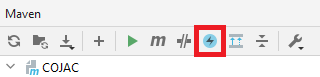
\includegraphics[width=.5\linewidth]{problems/maven_skip_tests.png}
}
\captionof{figure}{Bouton pour ignorer les tests}
\label{fig:problems_maven_skip_tests}
\end{minipage}

\subsection{Cause}

Dans un des fichiers de log produits, qui sont mentionnées dans la section \ref{sec:problems_surefire_problem}, on peut trouver l'erreur suivante:

\begin{minted}[breaklines]{text}
# Created at 2021-06-03T14:09:01.042
Error opening zip file or JAR manifest missing : D:\Documents\Documents\HEIA\Semestre
\end{minted}

Ce lien est incomplet par rapport au chemin mentionné dans la section \ref{sec:problems_surefire_problem}. Le chemin d'accès s'arrête lors du premier espace trouvé. Si le projet est déplacé dans un dossier ne contenant aucun espace, le \gls{JAR} est correctement généré.

\subsection{Solution}

Il faut modifier une ligne de configuration du plugin Surefire dans le \textit{pom.xml}. Des guillemets ont été ajoutés autour du chemin d'accès du \gls{JAR} pour obtenir la ligne suivante.
\inputmintedcolor[linenos=false,xleftmargin=0pt]{xml}{code/maven-surefire-javaagent.xml}

Ce changement corrige le problème.

\section{Erreur lors de l'instrumentation d'une application par COJAC}
\label{sec:problem_cojac_instrumentation}

Lors de l'appel de la commande pour instrumenter une démonstration avec \gls{COJAC}, \gls{COJAC} provoque une erreur.

\subsection{Problème}

L'application peut être démarrée sans \gls{COJAC} avec la commande suivante:
\begin{minted}{bat}
java demo\HelloBigDecimal.java
\end{minted}

Cependant, \gls{COJAC} produit une erreur lorsque l'application est démarrée avec \gls{COJAC}. La commande suivante a été utilisée:
\begin{minted}{bat}
java -javaagent:cojac.jar="-Rb 50" demo\HelloBigDecimal.java
\end{minted}

\subsection{Solution temporaire: compiler avec Java 8}

\gls{COJAC} doit être compilé avec Java 9 au minimum, mais l'application instrumentée doit être compilée avec Java 8. Les deux commandes suivantes permettent de compiler une démonstration et de l'exécuter:
\begin{minted}{bat}
javac -source 8 -target 8 demo\HelloBigDecimal.java
java -javaagent:cojac.jar="-Rb 50" demo.HelloBigDecimal
\end{minted}

\subsection{Cause}

La source du problème provient de l'instruction \gls{Bytecode} \textit{Invokedynamic} qui a évolué en Java 9 et qui est désormais utilisé pour de nouvelles opérations qui ne sont pas supportés par \gls{COJAC} à l'heure actuelle.

\section{Erreur des tests unitaires}

Lors de la création du \gls{JAR}, un test peut parfois échouer.

\subsection{Problème}

Un test déjà présent dans le projet et qui agit sur une autre partie du projet peut parfois créer une erreur. Lors de la création du \gls{JAR}, l'erreur suivante peut se produire:

\begin{minted}[breaklines]{text}
[ERROR] Failures: 
[ERROR]   Double2FloatTest.testDouble2FloatConversion:79 On "testNextUp", Got: 3.0000000000000004, Expected: 3.000000238418579
\end{minted}

Ce test agit sur les \textbf{\glspl{Behaviour}} alors que ce projet se focalise sur les \textbf{\glspl{Wrapper}}. Ces deux concepts distincts sont expliqués dans la section \ref{sec:cojac_integration}. Cette erreur est devenue un problème particulièrement important lorsqu'elle est devenue récurrente sur le GitLab CI alors qu'elle est invisible sur la machine de développement. Cette erreur complique la détection des autres erreurs sur le GitLab CI.

\subsection{Cause}

Lorsque l'instrumentation est effectuée, elle doit aussi remplacer certaines méthodes des librairies standards telles que \textit{Math.nextUp}. Cependant, il y a une condition qui peut éviter les méthodes d'être instrumentées qui peut être vue dans l'extrait de code suivant:
\begin{minted}{Java}
for(Method m:behaviorClass(i).getMethods()){
    if (m.isAnnotationPresent(UtilityMethod.class)){
        break;
    }
\end{minted}
Lorsqu'il y a une méthode qui est annotée, cette méthode et toutes les méthodes suivantes ne sont pas instrumentées.

\subsection{Solution}

Il semble plus logique de ne pas instrumenter la méthode possédant l'annotation uniquement. Pour ce faire, le code a été changé pour correspondre à l'extrait de code suivant:
\begin{minted}{Java}
for(Method m:behaviorClass(i).getMethods()){
    if (m.isAnnotationPresent(UtilityMethod.class)){
        continue;
    }
\end{minted}

Face à la difficulté de comprendre ce code, il est difficile de savoir si c'est vraiment la bonne correction. Cependant, l'erreur n'est plus réapparue depuis.

\subsection{Remarques}

Cette erreur était très difficile à trouver car elle ne se produisait pas sur la machine locale. Il a fallu ajouter des logs pour détecter la différence de comportement entre les deux environnements. De plus, le code est long et peu explicite. Il utilise également certaines mauvaises pratiques. Ainsi, cette erreur a permis de mettre en avant certains problèmes:

\begin{itemize}
    \item La classe \textit{com.github.cojac.instrumenters.BehaviourInstrumenter} peut et devrait être améliorée. Il y a beaucoup de code commenté, certaines méthodes sont très longues, il y a jusqu'à 6 niveaux d'indentations et l'apparition d'exceptions est considérée comme un cas habituel et n'est pas signalé.
    \item La classe \textit{com.github.cojac.instrumenters.BehaviourInstrumenter} contient d'autres \textit{break} suspicieux.
    \item Les tests du profiler produisent une grande quantité de texte sur la sortie standard. Ce texte n'a pourtant que peu d'intérêt.
\end{itemize}

\section{Erreur de compilation de \textit{SoftPosit}}
\label{sec:problem_softposit_compilation}

Après le téléchargement du dépôt de \gls{SoftPosit}, la compilation de la librairie provoquait une erreur.

\subsection{Problème}

La compilation de l'erreur provoque de nombreuses erreurs dans le fichier \textit{softposit.h} dont les premières sont disponibles ci-dessous.

\begin{minted}[breaklines]{Text}
In file included from ../../source/include/internals.h:50,
                 from ../../source/s_addMagsP8.c:38:
../../source/include/softposit.h:176:5: error: expected '=', ',', ';', 'asm' or '__attribute__' before '.' token
   uA.ui = ((uA.ui + mask) ^ mask)&0xFF;
     ^
../../source/include/softposit.h:177:5: error: expected '=', ',', ';', 'asm' or '__attribute__' before '.' token
   uA.p; \
     ^
../../source/include/softposit.h:178:1: error: expected identifier or '(' before '}' token
 })
\end{minted}

\subsection{Cause}

Ces erreurs se produisent à cause de certaines macros qui contiennent des lignes qui ne se terminent pas par le caractère \textbackslash. Ce caractère est indispensable car il permet de dire que le compilateur doit ignorer le retour à la ligne. Ceci permet ainsi d'indiquer que ces nouvelles lignes font partie de la macro.

\begin{minted}{C}
#define absP8(a)({\
		union ui8_p8 uA;\
		uA.p = (a);\
		int const mask = uA.ui >> 7;
		uA.ui = ((uA.ui + mask) ^ mask)&0xFF;
		uA.p; \
})
\end{minted}

\subsection{Solution}

\begin{minipage2}
Il suffit d'ajouter des \textbackslash {} à la fin de ces lignes pour corriger le problème.

\begin{minted}{C}
#define absP8(a)({\
		union ui8_p8 uA;\
		uA.p = (a);\
		int const mask = uA.ui >> 7; \
		uA.ui = ((uA.ui + mask) ^ mask)&0xFF; \
		uA.p; \
})
\end{minted}
\end{minipage2}

Un fork du projet a été créé pour corriger ce problème. Une merge request (\url{https://gitlab.com/cerlane/SoftPosit/-/merge_requests/7}) est actuellement en attente pour corriger ce problème sur le dépôt principal.

\section{Inclure \textit{SoftPosit} lors de la compilation de la librairie native}
\label{sec:problem_softposit_include}

Lors de la compilation de la librairie avec Ubuntu, une erreur était générée lors de l'ajout de la librairie \gls{SoftPosit}.

\subsection{Problème}

Lors de la compilation de la librairie qui fait la passerelle entre \gls{JNI} et \gls{SoftPosit}, l'erreur suivante était produite:

\begin{minted}[breaklines,breakanywhere]{Text}
/usr/bin/ld: src/libraries/SoftPosit/build/Linux-x86_64-GCC/softposit.a(p32_sqrt.o): relocation R_X86_64_PC32 against symbol `softposit_approxRecipSqrt1' can not be used when making a shared object; recompile with -fPIC
/usr/bin/ld: final link failed: bad value
\end{minted}

\subsection{Cause}

Cette erreur signifie que \gls{SoftPosit} a été compilée pour être à un endroit précis. Cependant, lorsque \textit{SoftPosit} est ajoutée dans la librairie, le compilateur a besoin de changer les adresses.

\subsection{Solution}

Il faut modifier le \gls{Makefile} de \gls{SoftPosit}. Dans l'ancien \gls{Makefile}, il y avait cette ligne:

\inputmintedcolor[linenos=false,xleftmargin=0pt]{Makefile}{code/softposit_old_Makefile}

\begin{minipage2}
Il faut ajouter l'option \textit{-fPIC} afin d'obtenir la ligne suivante:

\inputmintedcolor[linenos=false,xleftmargin=0pt]{Makefile}{code/softposit_current_Makefile}
\end{minipage2}